\documentclass[tikz,border=0pt]{standalone}
\usepackage[dvipsnames]{xcolor}
\usetikzlibrary{matrix,fit}

\begin{document}
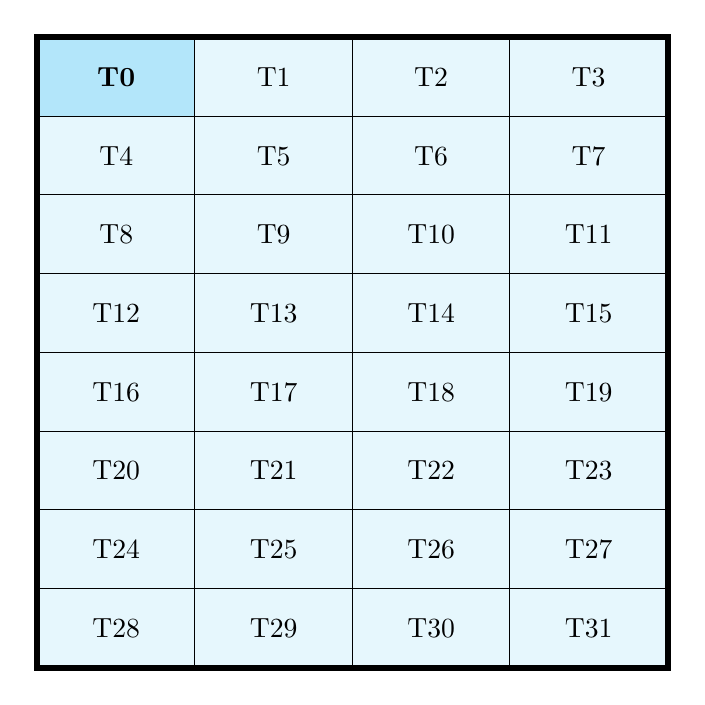
\begin{tikzpicture}[%
    mymatrix/.style={%
        matrix of nodes,
        nodes in empty cells,
        row sep=-\pgflinewidth, % [[5]] 避免双线
        column sep=-\pgflinewidth,
        nodes={%
            draw,
            minimum height=1cm,
            minimum width=2cm,
            anchor=center,
            fill=cyan!10,
%           fill=CornflowerBlue!15,
            text=black,
            %outer sep=0pt,
            inner sep=2pt,
        },
        execute at empty cell={\node {};} % [[5]] 填充空单元格
    }
]
\matrix[mymatrix] (mat) {
    |[fill=cyan!30,font=\bfseries]|
    T0 & T1 & T2 & T3 \\
    T4 & T5 & T6 & T7 \\
    T8 & T9 & T10 & T11 \\
    T12 & T13 & T14 & T15 \\
    T16 & T17 & T18 & T19 \\
    T20 & T21 & T22 & T23 \\
    T24 & T25 & T26 & T27 \\
    T28 & T29 & T30 & T31 \\
};

% 绘制外层边框
\node[draw,line width=2pt,inner sep=0pt,fit=(mat-1-1)(mat-8-4)] {};

\end{tikzpicture}
\end{document}
